\chapter{Methodology}
\label{methodology}

\section{Project management methodology}
I will use a cyclical, evolutionary method. This will involve:
\begin{itemize}
  \item Requirements elicitation.
  \begin{itemize}
    \item This involves determening the needs of the user and defining requirements to meet those ends.
  \end{itemize}
  \item Feature design (UI).
  \begin{itemize}
    \item Features will be designed at first using wireframe models. Then on later iterations, colour and shading will be added alongside further usability considerations such as highlight on hover etc.
  \end{itemize}
  \item Feature implementation research.
  \begin{itemize}
    \item This step involves determining the apropriate technologies and libraries to achieve the design. This is nececarry to realize the constraints that are imposed by the implementation method and know to what extent the design is feasible.
  \end{itemize}
  \item Feature implementation.
  \begin{itemize}
    \item Writing the code to create the feature.
  \end{itemize}
  \item Feature testing.
  \begin{itemize}
    \item Initially testing will be done manually with valid values until later iterations whereby extraneous values will be introduced. Once the feature is in it's final iterations a unit test will be introduced.
  \end{itemize}
  \item Evaluation.
  \begin{itemize}
    \item Does the feature meet the requirements and fulfill the needs of the user?
  \end{itemize}
\end{itemize}
This workflow will consist of a single cyclical workflow, with two nested "sub workflows" whereby upon completion of a step, it is sometimes nececarry to loop back on oneself to perform futher refinement. As illustrated by the diagram below.
\begin{figure}
  \begin{center}
    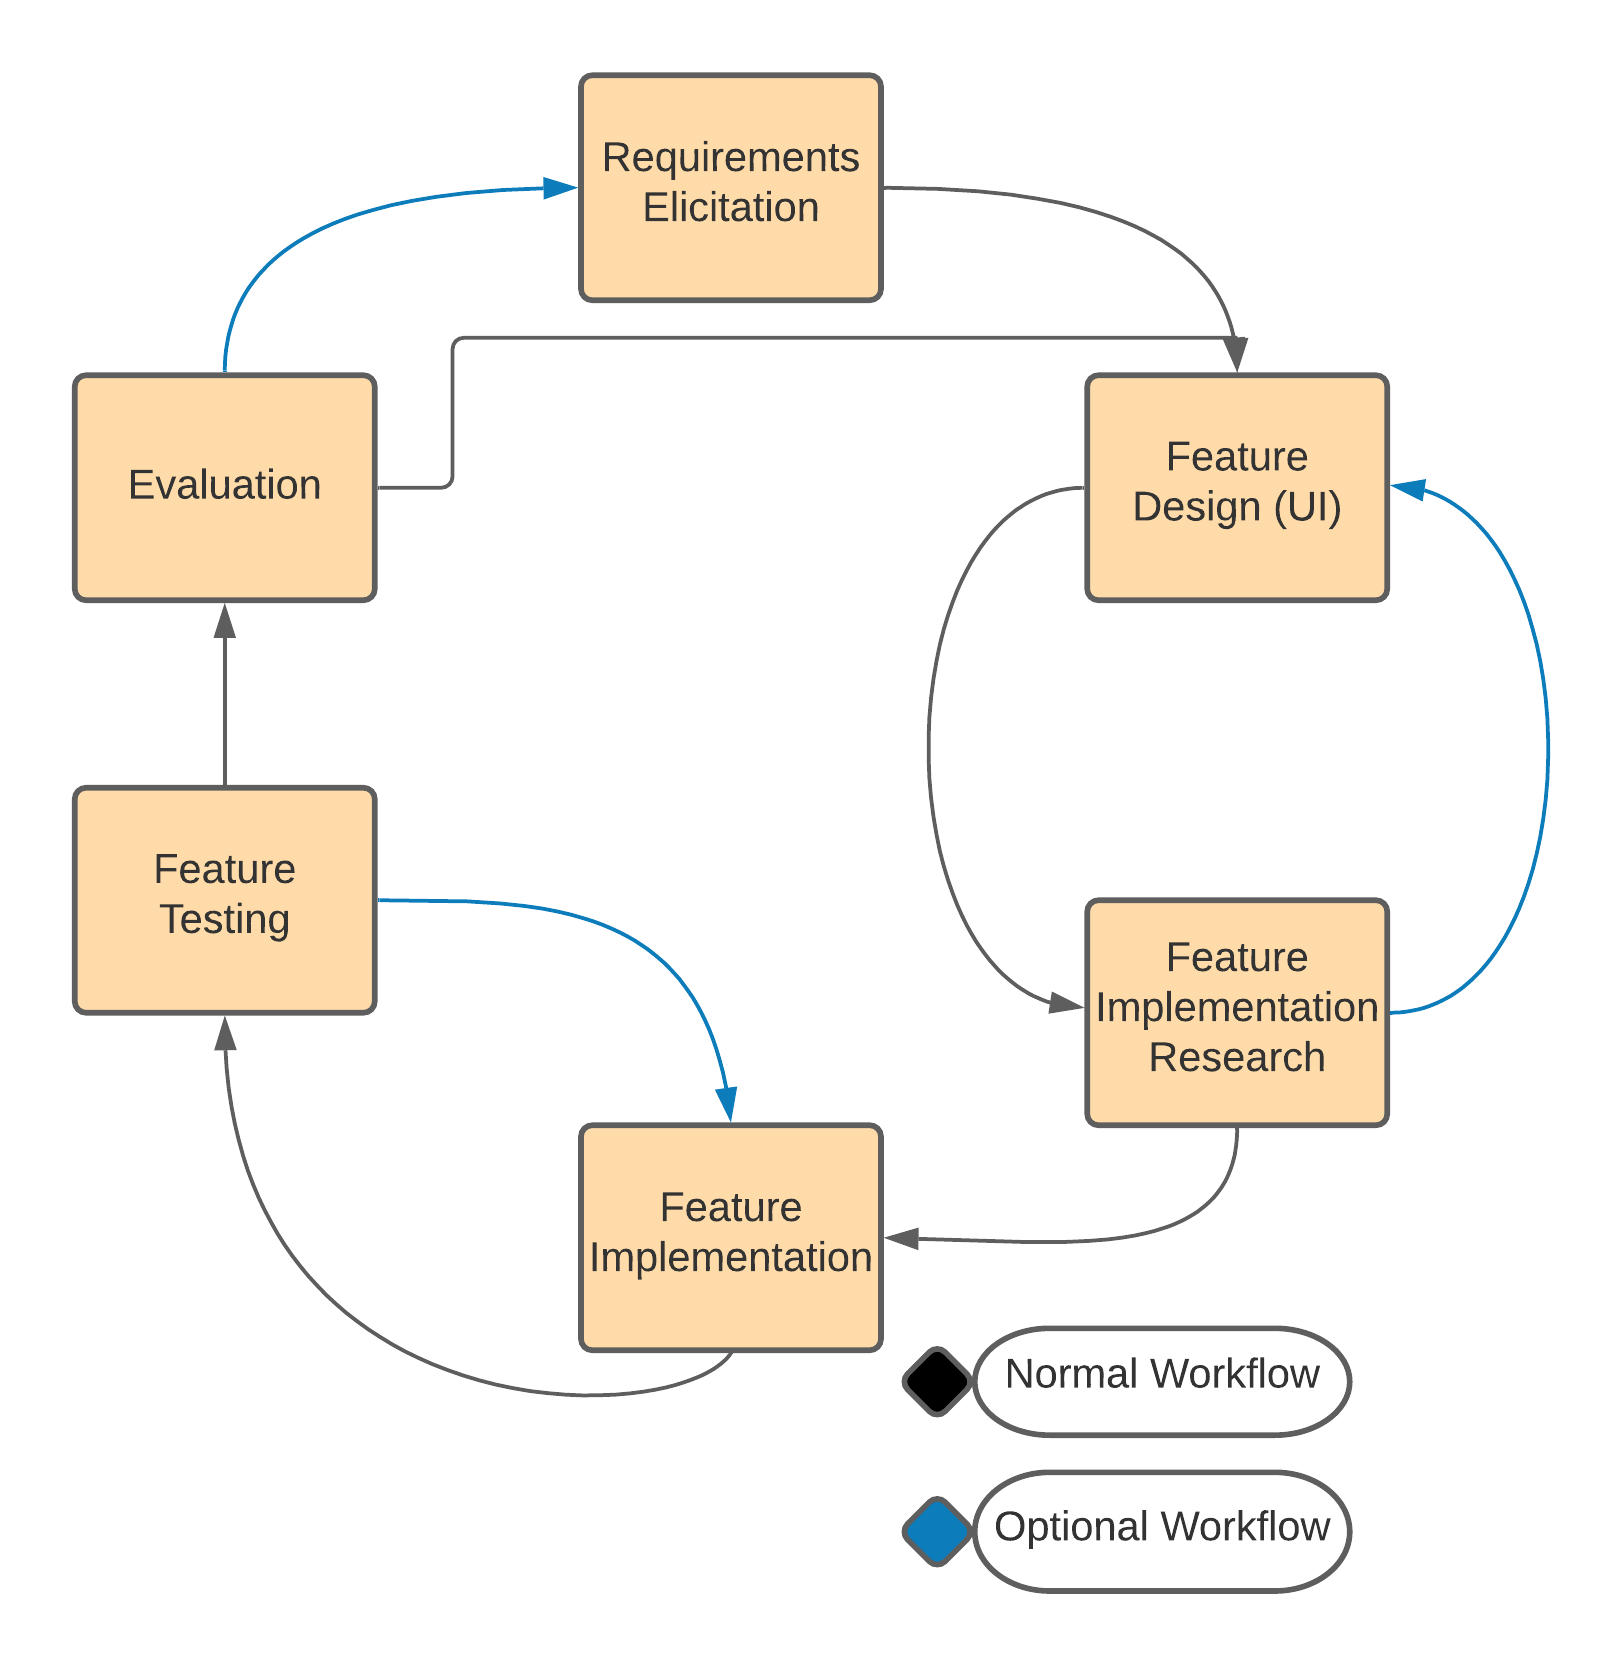
\includegraphics[scale=0.75]{Images/Project_Management_Methodology}
    \caption{Development Lifecycle}
    \label{fig:development lifecycle}
  \end{center}
\end{figure}
Throughout the project the focus of the workflow will shift as illustrated by the diagram below.

\begin{figure}
  \begin{center}
    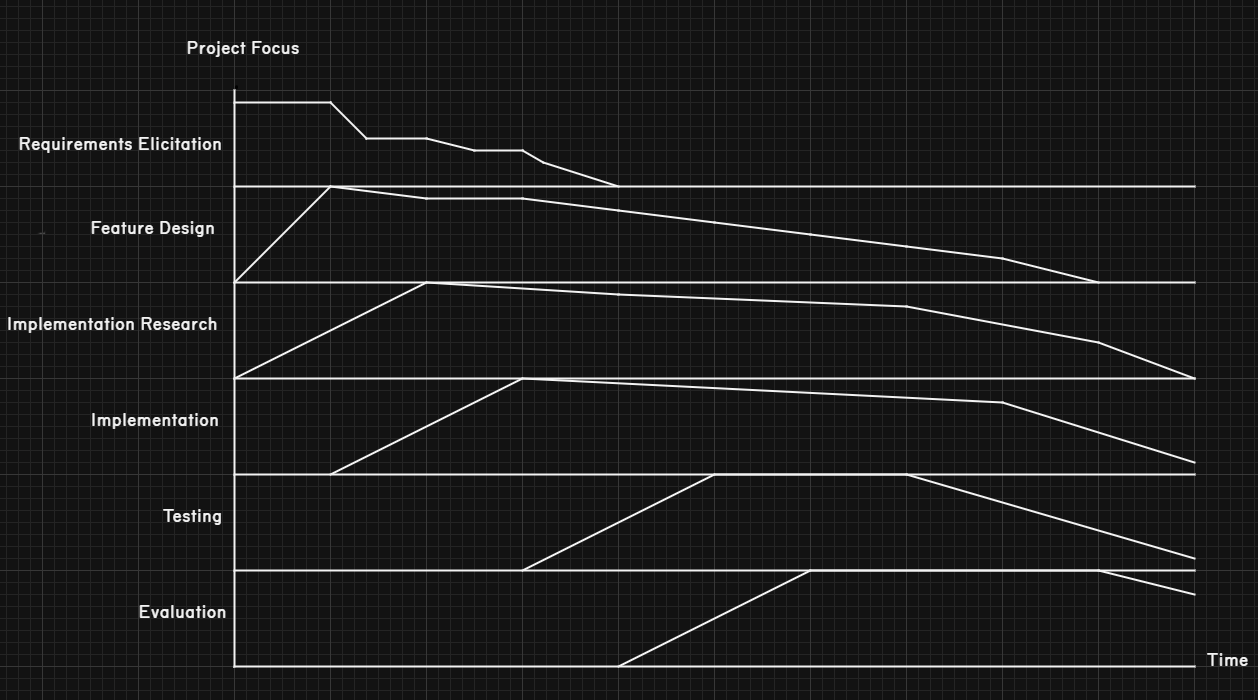
\includegraphics[scale=0.4]{Images/ProjectFocus2}
    \caption{Project Focus Over Time}
    \label{fig:project focus}
  \end{center}
\end{figure}
\section{Evaluation Design}
 (what method(s), used how, with what and how many participants?)

\section{Requirements Elicitation}
  How will requirements of the software be determined.

\section{Feature management}
  To track the creation and completion of features, a Kanban board will be used. This will include columns for 'To do', 'Doing' and 'Done'.

\section{Design Methods}
   (e.g., wireframes, DFDs, use case diagrams, class diagrams, sequence diagrams, ERDs, etc)

\section{Testing methods}

\section{Version control}
  I will be using Git and Github. This will allow the creation of branches to explore experimental parts of the soloution space without disrupting the progress of the main branch. If the experimental implementation is successfull it will be merged with the main branch. It also allows the development of features in paralel, with any conflicts in their implementation being resolved at the merge stage. The inclusion of a remote repository allows for work to continue on a seperate machine if nececarry and later be synced with the local main branch.
  \begin{figure}[H]
    \begin{center}
      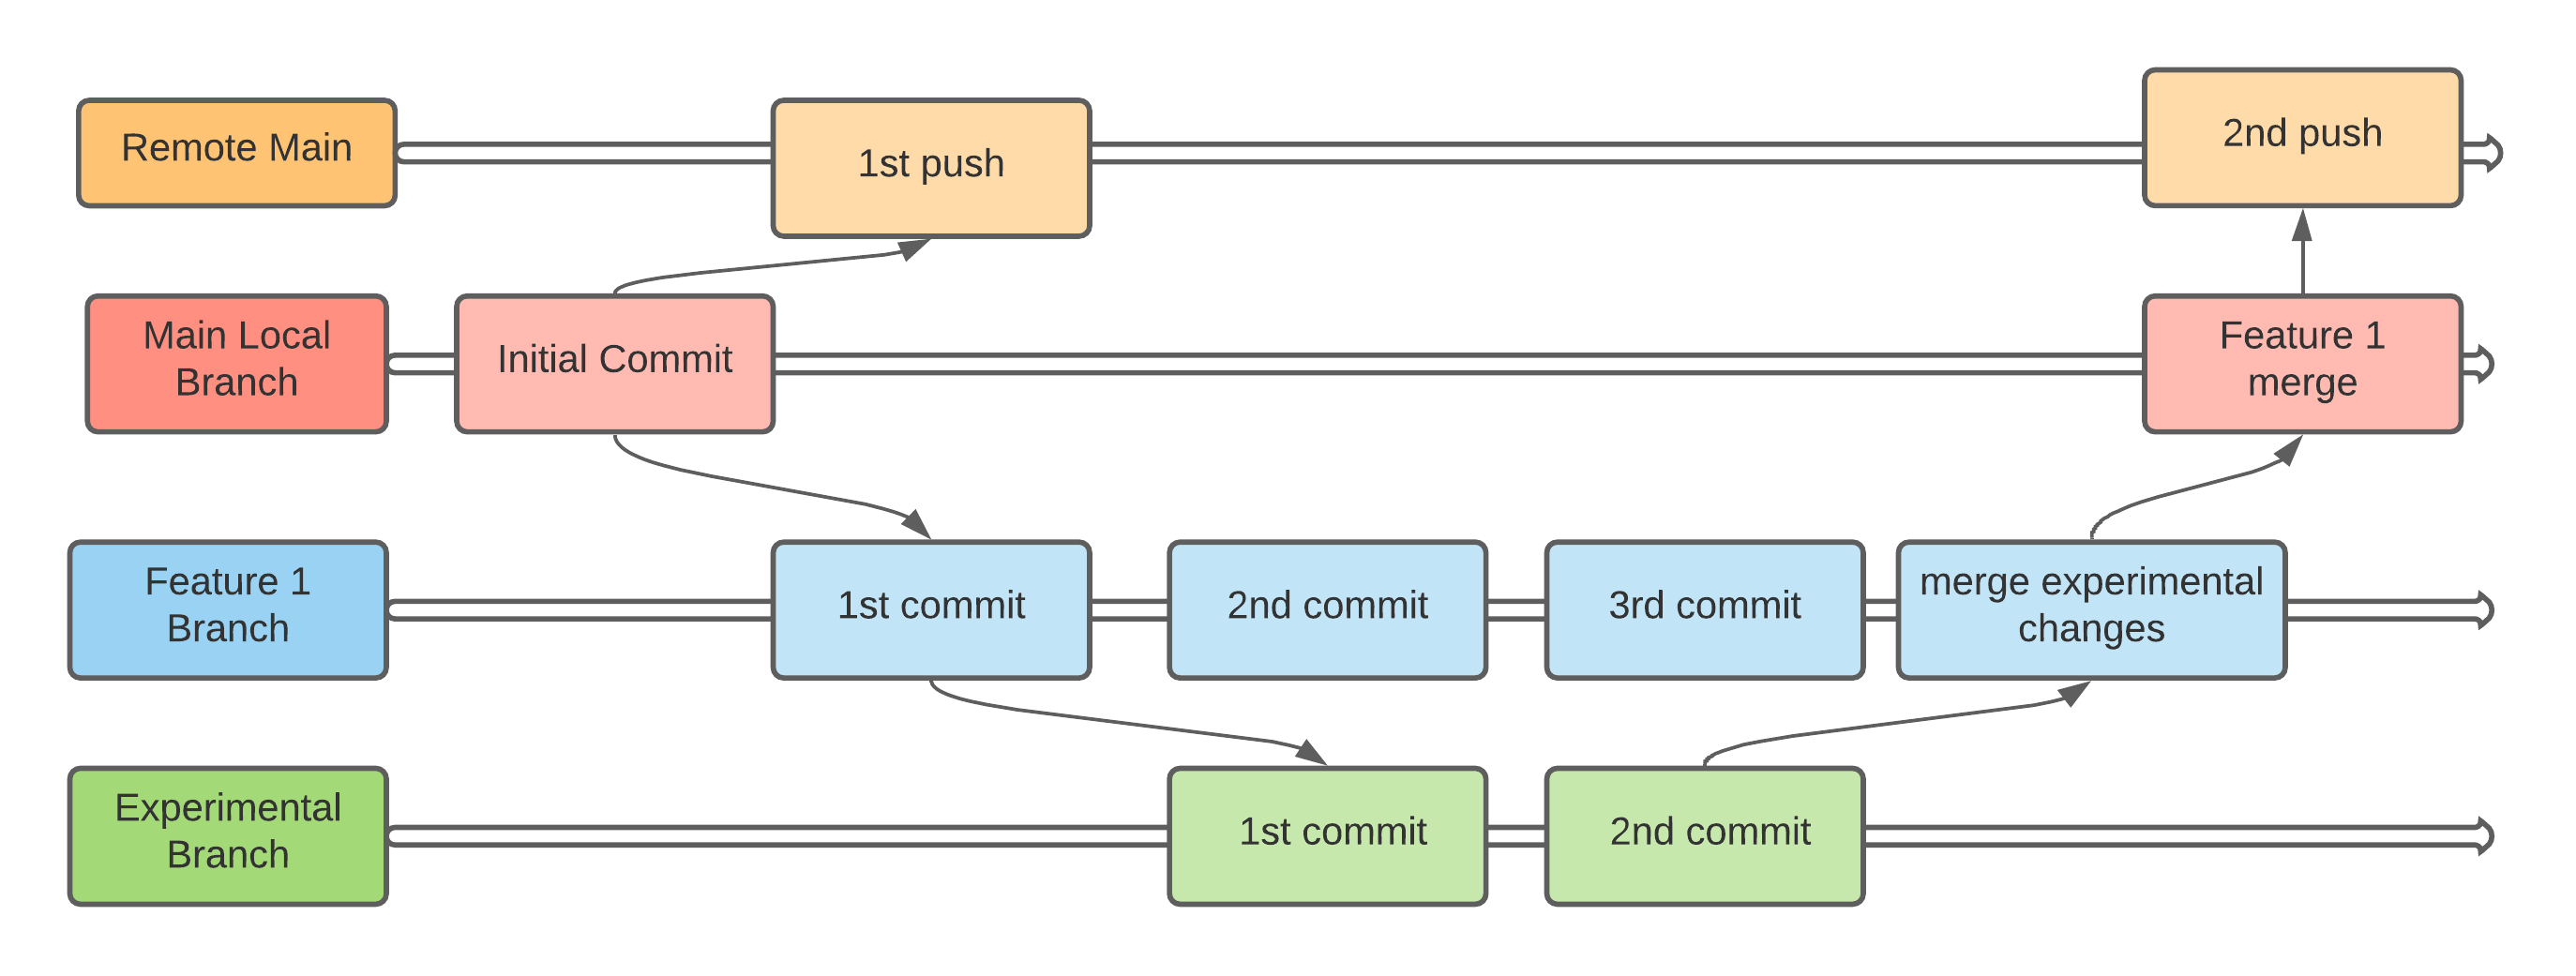
\includegraphics[scale=0.7]{Images/Git_Workflow_Diagram}
      \caption{Example Workflow To Highlight Branch Usage}
      \label{fig:Git Workflow}
    \end{center}
  \end{figure}

\section{Evaluation methods}
  e.g. SUS (system usability scale)

\section{Requirements}
  TEST TEXT
\section{Desing and Implementation details}

\section{Justification of Implementation Choices}
